% Cos'è

Web search has evolved since it was a massive link analysis system. Now the
contents of a search query has been enriched with multimedia contents from the
crowd. For instance a query can show results as links to other websites,
user generated video, tweets or images. On top of this, a lot of tasks has been
tweaked to generate more searchable data (e.g. image and video tagging), so now
we are able to search for them. The crowd is becoming part of the search process,
by adding information, ranking the results, moderating contents, etc.\\

CrowdSearch is targeted to enabling, promoting and understanding individual
and social participation to search \cite{fraternali2012crowdsearch}.
CrowdSearch uses the crowds as sources for the content processing and information
seeking processes; it fills the gap between generalized search systems, which
operate upon world-wide information - including facts and recommendations as
crawled and indexed by computerized systems { and social systems, capable of
interacting with real people, in real time \cite{fraternali2012crowdsearch}.
Crowd-searching can be defined as the promotion of individual and social participation
to search-based applications and improve the performance of information
retrieval algorithms with the calibrated contribution of humans \cite{paperboz}.



\subsubsection{The CrowdSearch framework}
\begin{figure}[htb]
    \centering
    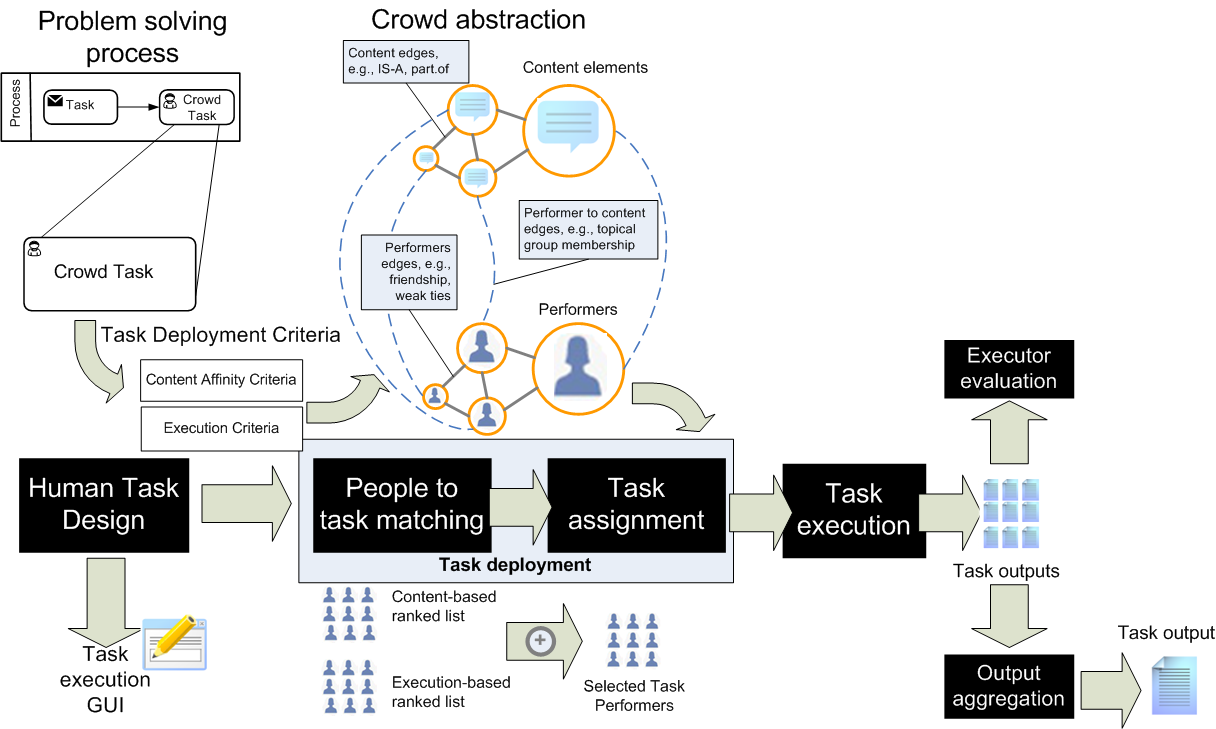
\includegraphics[width=\columnwidth]{CS-framework}
    \caption{The CrowdSearch framework.}
    \label{fig:CS-framework}
\end{figure}
The framework (see \autoref{fig:CS-framework}) proposed by \cite{paperboz}, uses the
humans' skills to improve some the result of a query. To perform such operation
the framework must choose which task must be executed by humans and which must
not. This has been addressed by mapping some task to humans and some to machines.

When a task is assigned to the crowd, the execution mode is chosen according to
the \emph{Human Task Design}. This step produces the actual design of the
\emph{Task Execution GUI}, and the \emph{Task Deployment Criteria}.
These criteria can be logically subdivided into two subject areas: \emph{Content
Affinity Criteria} (what topic the task is about) and \emph{Execution Criteria}
(how the task should be executed). The Execution Criteria could specify constraints
or desired characteristics of task execution including: a time budget for
completing the work, a monetary budget for paying workers, etc.

The framework provides an abstraction for the crowd and their skills, called
\emph{Crowd Abstraction}, human performers and content elements are represented
as nodes connected by edges in a bipartite graph.
Edges connecting performers denote a friendship, edges connecting content
elements denotes a semantic relationships and finally, a connection from a
performer to a content element may denote an interest.

The next step to the \emph{Human Task Design} is the \emph{Task Deployment}, whose
goal is to assign the crowd tasks to the most suited performers. This step is
subdivided in two sub-step: \emph{People to Task Matching} and \emph{Task
Assignment}. The first sub-step is almost a query matching problem, where the
workers must be ranked according to the \emph{Task Deployment Criteria} and a
set of suitable workers is selected (e.g. top-k).

The final step is the \emph{Task Execution}. This step is the actual execution
of the task by the crowd. The results are then merged to form the result of the
crowd task.